\section{АНАЛІЗ РИНКУ І ПОТОЧНИХ РІШЕНЬ}
На даний момент існує досить багато готових рішень корпоративних порталів. 
Вони можуть забезпечувати підприємства всіма необхідними функціями і додатками, починаючи від системи обліку працівників, і завершуючи системою аналітики і збору даних, все це залежить від потреб ринку і певної компанії.
Проте майже всі вони здебільшого призначені для великих компаній, і невеличкі компанії або повинні витрачати величезні гроші на покупку ліцензій, або ж не користуватися усіма перевагами корпоративного порталу.
Тому було проведено загальний огляд продуктів і виділено основні переваги і недоліки, також виділено поточну використовувану ліценцію розповсюдження ПЗ.
\subsection{Переваги та недоліки поточних рішень}
Зробивши аналіз даної сфери, можна виділити декілька основних аспектів, які будуть використані для розробки подальшого програмного продукту.
Левова частка програмного забезпечення корпоративних порталів розроблено згідно стандартів\cite{portlet_2}. 
Всі додатки і аплікації можуть без проблем взаємодіяти між собою. 
Проте великою їх нестачею для малої сфери бізнесу є закритість програмного коду і величезна вартість ліцензій.
Тому невеличкі компанії (до 100 людей) просто не мають змоги собі дозволити таку <<розкіш>>.

\subsubsection{Ліцензіювання і відкритість АРІ}
\par Було проведено аналіз поточних продуктів і їх ліцензій, і виявлено, що майже 90\% використовує проприєтарні рішення.
Більш детально розглянуто у таблиці \ref{t:portals}:

\begin{center}\footnotesize
\begin{longtable}{|c|c|c|}
\captionsetup{justification=centering}
\caption{Список корпоративних порталів і використовувана ліцензія}\label{t:portals}\\
\hline
\multicolumn{1}{|c|}{\textbf{Назва продукту}}&
\multicolumn{1}{c|}{\textbf{Технологія}}&
\multicolumn{1}{c|}{\textbf{Ліцензія}}\\\hline

\endfirsthead
\caption*{\hfill Продовження таблиці \ref{t:portals}}\\\hline

\multicolumn{1}{|c|}{\textbf{Назва продукту}}&
\multicolumn{1}{c|}{\textbf{Технологія}}&
\multicolumn{1}{c|}{\textbf{Ліцензія}}\\\hline
\endhead

Jetspeed & Java EE & Apache License v2.0\\ \hline
 ATG Portal & Java EE & Proprietary\\ \hline
 Backbase Portal Software & Java EE, .NET & Proprietary \\ \hline 
 Broadvision Portal & Java EE & Proprietary \\ \hline 
 Bluenog ICE & Java EE & Proprietary \\ \hline
 enPortal  & Java EE & Proprietary\\ \hline 
 CommunityManager.NET  & .NET & Proprietary \\ \hline
 eXo Portal & Java EE & Affero General Public License \\ \hline
 eXo Platform & Java EE & Proprietary \\ \hline
 GateIn Portal & Java EE & LGPL \\ \hline
 Hippo CMS & Java EE & Open Source and Proprietary Licenses \\ \hline
 WebSphere Portal & Java EE & Proprietary \\ \hline
 TeamPortal & Java EE & Proprietary \\ \hline
 JBoss Enterprise Portal  & Java EE & LGPL \\ \hline
 IntraNet & ASP.NET & Proprietary \\ \hline
 Liferay Portal & Java EE & Proprietary Licenses \\ \hline
 TeamWox Groupware & C++ & Proprietary \\ \hline
 SharePoint Server & ASP.NET & Proprietary \\ \hline
 Vignette Portal 8.0 & Java EE & Proprietary \\ \hline
 Oracle WebCenter Suite 11g & Java EE & Proprietary \\ \hline
 Oracle WebLogic Portal 10g & Java EE & Proprietary \\ \hline
 Oracle WebCenter Interaction 10g & ASP.NET & Proprietary \\ \hline
 Oracle IAS Portal 10g & Java EE & Proprietary \\ \hline
 Regroup & Ruby & Proprietary \\ \hline
 ACUBE Portal 5.0 & Java EE & Proprietary \\ \hline
 SAP NetWeaver 7.0 & Java EE & Proprietary \\ \hline
 SORCE V9 & ASP.NET & Proprietary \\ \hline
 Sun Java System Portal Server & Java EE & Open Source, licensing \& support plans \\ \hline
 Sun GlassFish Web Space Server  & Java EE & Open Source, licensing \& support plans \\ \hline
 tmsEKP 1.52 & Java EE & Proprietary \\ \hline
 PortalBuilder 5.2 & Java EE & Proprietary \\ \hline
 ProPortal 4.0 & Java EE & Proprietary \\ \hline
 Intrexx & Java EE & Proprietary \\ \hline
 uPortal & Java EE & Apache License v2.0 \\ \hline

\end{longtable}
\end{center}


Зробивши певний аналіз, можна дійти до висновку, якби невеликим компаніям давати можливість використовувати продукт на підставах вільного розповсюдження коду, то вони б охотніше пробували, і з часом інвестували в нього гроші, або просто <<купляти>> підтримку.
Тобто використати одну із відкритих ліцензій типу GNU Public License.
\par Економічна вигода продукту буде базуватися на корпоративній платній підтримці, типу все починаючи від підбору серверів --- до налаштування і підтримки продукту.
Зате розробники зможуть у загальний репозиторій додавати свої зміни та виправляти помилки, що значною мірою пришвидшить процес розробки.
Основна стратегія розробки буде націлена на швидкий вихід на ринок і пошук потенційних клієнтів.
Також велика увага буде прикута для ринку пост радянських республік, адже на даний момент ринок бізнесу стрімко розвивається, тобто попит є, а пропозиція не повній мірі відповідає потребі.
Портали які розробляються переважно націлені на Європейський та Американській ринок, а також Азію.
Тому базуючиь на цьому було виділено такі основні вимоги, як врахування нашого законодавства (для прикладу по працевлаштуванню працівників, ведення документації, конвертації валют і тому подібне) та локалізацію сервісу.
Тим більше підримка користувачів буде набагато легше і ефективніше всередині країни, ніж з-за кордону, що дасть нам перевагу над іншими існуючими продуктами.

\par Також велику увагу буде приділено відкритості АРІ для взаємодії із вже існуючими додатками.
Адже існуючі рішення в основному базуються на закритих протоколах, чим саме змушують користувачів прив'язуватися до їхньої системи і залежати від них
\par Інтерфейс і система всіх сучасних продуктів дуже <<важкиа>> і мульти-функціональна, що потребує значних ресурсів як у користувачів так і на стороні сервера.
Цей аспект також буде максимально спрощений, що в свою чергу дозволить виділитися продукту на ринку малого бізнесу.

\subsection{Технілогії розробки} 
Базуючись на поточних стандартах \cite{portlet_2} та використовуваних базових технологій (таблиця \ref{t:portals}) було прийнято рішення впровадити розробку на базі Java.
Адже саме Sun (зараз Oracle) <<диктує>> моду на ринку стандартизації портлетів, тому буде просто пристосуватися до поточних рішень.
\par Звичайно ж буде використано всі переваги Java EE.
Для гнучкої і швидкої розробки буде застосовано Spring Framework із ORM обгорткою Hibernate поверх бази даних MySQL.
Для фронт-енд логіки UI в основному буде використовуватися jQuery фреймоврк.
Пошук забезпечить Apache Lucene.
Сервер бек-енду буде працювати на Apache Tomcat.
\par На даний момент не планується стандартизація щодо портлетів, просто в майбутньому можливо буде виділено цей пункт для реалізації в системі.


\subsection{Технічний огляд продукту}
Розглянемо більш детально пункт про наявність сучасних засобів ведення бізнесу. 
Кожна компанія, завжди стикається із проблемою ведення обліку працівників, ведення обліку фінансів, спільної роботи над документами та іншим.
Також є величезна і невід'ємна потреба у спільному доступі до документів, до корпоративного календаря, до блогу користувачів, до електронних таблиць та інформаційної дошки.
\par Портал підприємства (також відомий як enterprise information portal (EIP) або корпоративний портал) є основою для інтеграції інформації, людей і процесів в рамках організації. 
Це дає змогу забезпечити єдину точку доступу, часто у вигляді веб-інтерфейсу і призначеної для агрегування та персоналізації інформації за допомогою конкретних програмних додатків. Однією відмінною рисою корпоративних порталів є децентралізоване внесення контенту та управління, яка зберігається на віддаленому сервері та постійно оновлюється.
%TODO змінити якось =)
\subsection{Історичний огляд корпоративної сфери}
В середині 1990-х років появилися громадські такі веб-портали як AltaVista, AOL, Excite і Yahoo!. 
Вони забезпечували користувачів певним набором функцій (наприклад новини, електронна пошта, погода, котирування акцій і пошук), які часто були представлені у вигляді автономного порталу.
Незабаром підприємства усіх типів і форм почали бачити необхідність аналогічного функціоналу для їх різноманітних потреб, проте із єдиною точкою доступу.
До кінця 1990-х років, виробники програмного забезпечення почали розробляти веб-портали для різних підприємств. 
Ці програмні пакети були розроблені таким чином, щоб підприємства могли легко розгортати свої власні налаштування корпоративного порталу та доповнювати його своїми додатками.
Перші постачальники комерційних веб порталів з'явилися в 1998 році, це були такі фірми як: Epicentric, Plumtree  та Viador. 
Ці фірми були основними гравцями на ринку, проте ситуація змінилася в 2002 року, коли на ринок почали виходити постачальники серверних аплікацій, такі як BEA, IBM, Passageways, Oracle Corporation and Sun Microsystems.
Підприємства можуть вибрати для своїх цілей декілька порталів, що базується на основі їх бізнес-структури та стратегічної спрямованості.
У 2003 році розробники Java-порталів випустили стандарт, відомий як JSR-168. 
Він повинен був визначити API для взаємодії між корпоративних порталів та портлетів.
Постачальники програмного забезпечення почали розробляти JSR-168 сумісні портлети, які можуть бути розгорнуті на будь-якому JSR-168 сумісному корпоративному порталі. 
Другий ітераційний стандарт JSR-286 є остаточним на даний момент і випущений 12 червня 2008 року.

\subsection{Портлети}
Портлет - це змінний компонент інтерфейсу веб-порталу (елемент веб-сторінки), який можливо певним чином підключити до порталу.
Портлет містить в собі фрагменти розмітки, які вбудовуються в сторінку порталу. 
Найчастіше сторінка порталу представляється у вигляді набору портлетів, які взаємодіють між собою. 
Таким чином, портлет (або сукупність портлетів) представляється у вигляді єдиного веб-додатку, розміщеного на порталі. 
Приклади портлетів можуть бути наступними: електронна пошта, повідомлення про погоду, фінансовий стан, останні новини і тому подібне.
Завдяки існуючим стандартам розробники можуть створювати портлети, що легко вбудовуються в будь-який портал, який слідує стандартам і правилам.
\par Існує протокол WSRP, що забезпечує стандарт веб-сервісів, що дозволяє автоматично вбудовувати віддалено запущені портлети з різних джерел.
Специфікація Java-портлетів JSR168 дає можливість взаємодіяти між собою портлети з різних веб-порталів. 
Ця специфікація визначає безліч API для взаємодії контейнерів портлетів і дає різні адреси областей персоналізації, подання та безпеки.
Існує безліч постачальників комерційних контейнерів портлетів. 
Як відомо лідирують у цій галузі IBM, Oracle, Vignette. 
Реалізації від цих постачальників мають додаткові розширення і налаштування, проте деякі із ним можуть бути не затверджені стандартами. 
Крім того, є портали з відкритим вихідним кодом, що підтримують JSR168, такі як корпоративний портал Apache Jetspeed-2 або eXo Portal.
\subsubsection{Apache Pluto}
Розглянемо на прикладі один з найбільш вдалої реалізації стандарту портлетів JSR168 - це Apache Pluto.
Портлет працює всередині контейнера портлетів (Pluto).
Цей контейнер містить портлет з необхідним середовищем для подальшого виконання.
Контейнер портлетів керує життєвим циклом всіх вікон порталу та надає інтерфейси для портлетів, котрі викликаються всередині нього.
Контейнер також запускає методи на виконання із доступних цільових користувацьких сторінок, і взаємодіє із сторінками порталу.  

    \begin{center}
		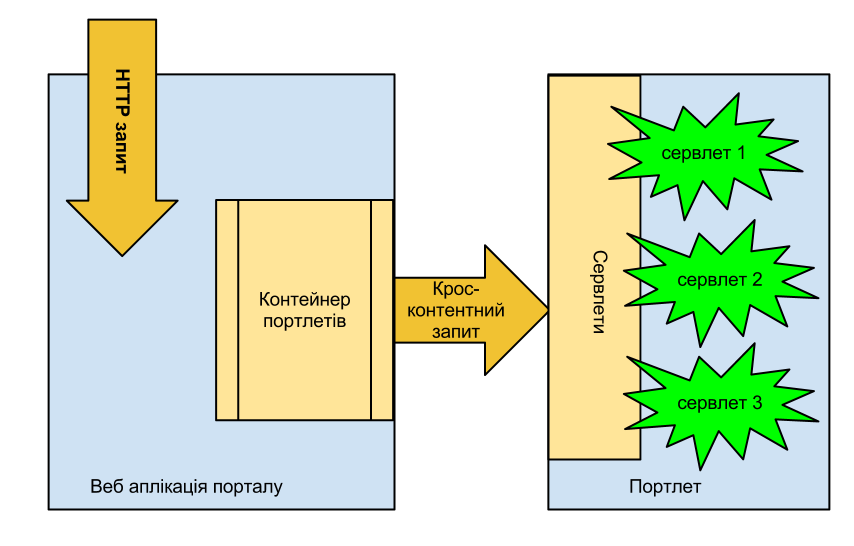
\includegraphics[width=1.00\textwidth]{pluto.png}
		\captionof{figure}{Принцип роботи <<Pluto>>}
	\end{center}

На наступному малюнку зображено архітектурні компоненти аплікації Pluto 2.0. 
\par В даному випадку, Pluto вбудований безпосередньо в корпоративний портал. 
Потім через перехресний запит (через веб-додатки) відбувається відправлення запиту для відображення вмісту портлету, який як правило знаходяться в різних додатках на порталі і в контейнерах. 


%TODO хз чи тут потрібно загальний розділ, поки забрав
\subsection{Система керування вмістом}
Система управління контентом (content management system - CMS) дозволяє публікувати, редагувати і змінювати вміст веб-сторінок, а також обслуговувати портал з центральної сторінки. 
При цьому надається набір процедур, що використовуються для управління робочим процесом у середовищі для спільної роботи.
Вони можуть бути ручні або комп'ютеризовані (в автоматичному режимі).
\subsubsection{Головні функції CMS}
До основних функцій можна віднести наступні пункти:
\begin{enumerate}
\item можливість великій кількості людей ділитися інформацією і робити свій вклад в розвиток порталу;
\item контроль доступу до даних на основі ролей користувачів (наприклад визначити роль, яка має тільки права на перегляд інформації, або ж редагування, публікацію тощо);
\item пошук і поширення інформації між користувачами;
\item зменшення дублікацій на вході;
\item спрощене керування корпоративними додатками;
\item відносно легка комунікація між користувачами.
\end{enumerate}

\subsubsection{Типи даних та їх використанням}
У CMS дані можуть бути представлені як правило у будь-якій формі: документи, відео, тексти, фотографії, номери телефонів, наукові дані і тому подібне. 
CMS часто використовуються для зберігання, управління, перегляду і публікації документів. 
Також досить поширене використання в якості центрального сховища у зв'язці із централізованою системою контролю версій, що є однією із переваг CMS.
\subsubsection{Управління корпоративною інформацією}
Enterprise Content Management (ECM) - управління інформаційними ресурсами підприємства або управління корпоративною інформацією.
В даному контексті інформація (контент) передбачається як слабо структурована одиниця - це можуть бути файли різних форматів, електронні документи з різними наборами полів і т. п.
За визначенням ECM - це стратегічна інфраструктура і технічна архітектура для підтримки єдиного життєвого циклу неструктурованої інформації різних типів і форматів. 
ECM-системи складаються з додатків, які можуть взаємодіяти між собою, а також використовуватися і продаватися самостійно. 
\par Всі сучасні ECM-системи визначають такі ключові компоненти:
\begin{enumerate}
\item управління документами --- довгострокове архівування, автоматизація політик зберігання та відповідності нормам регулюючих органів, забезпечення відповідності законодавчим та галузевим нормам;
\item управління веб-контентом (WCM) --- автоматизація ролі веб-майстра, управління динамічним контентом і взаємодією між користувачами;
\item  управління мультімедіаконтентом (DAM) --- управління графічними, відео та аудіофайлами, різними маркетинговими матеріалами, наприклад, флеш-банерами, рекламними роликами;
\item управління знаннями (Knowledge Management) --- підтримка систем для накопичення та доставки релевантної для бізнесу інформації;
\item документо-орієнтоване взаємодія (співробітництво) --- спільне використання документів користувачами та підтримка проектних команд.
\end{enumerate}

%TODO якщо буде мало тексту, вставити http://en.wikipedia.org/wiki/Enterprise_content_management
%\subsubsection{Компоненти ECM} 

\subsection{Система управління документами}
Система управління документами (DMS - Document management system) - комп'ютерна система (або набір комп'ютерних програм), що використовується для відстеження та зберігання електронних документів і / або образів (зображень та інших артефактів) паперових документів.
Дане поняття тісно пов'язане з концепцією Content Management System (система керування вмістом) і зазвичай розглядається як компонент Enterprise Content Management System (CMS рівня підприємства).
У загальному випадку системи управління документами (DMS) надають можливість зберігання, ведення контролю версій, позначення метаданими і безпеку по відношенню до документів, а також індексування і розвинені можливості пошуку документів.
\subsubsection{Метадані}
Метадані зазвичай зберігаються для кожного документа. 
Метадані, наприклад, можуть включати дату занесення документа в сховище і код користувача, котрий виконав зміни до файлу. 
Система управління документами також може витягувати метадані з документа автоматично або запитувати їх у користувача. 
Деякі системи надають сервіс оптичного розпізнавання тексту відсканованих документів, або можливість витягувати текст з електронних документів. 
Використовуючи опрацьований текст система дозволяє здійснювати пошук документа за ключовими словами всередині самого документа.

\subsubsection{Інтеграція }
Багато систем управління документами намагаються інтегрувати функцію управління документами безпосередньо в різні додатки, дозволяючи користувачеві отримувати документ відразу зі сховища системи управління документами, робити які-небудь модифікації, і зберігати його назад в сховище в якості нової версії, і все це проробляти в одному додатку, не виходячи з нього. 
Дана інтеграція в основному доступна для офісних пакетів і поштових клієнтів або для програмного забезпечення, призначеного для групової або колективної роботи. 
Інтеграція зазвичай має на увазі використання таких відкритих стандартів як: ODMA, LDAP, WebDAV і SOAP.

\subsubsection{Захоплення тексту}
Під захопленням тексту мається на увазі переведення паперових документів в цифровий варіант за сканерів та МФУ.
Також часто використовується програмне забезпечення для оптичного розпізнавання тексту, щоб конвертувати цифрові зображення в текст.

\subsubsection{Індексування}
Індексування надає можливість класифікувати документи за допомогою метаданих і індексування словникового тексту, який було витягнутого з документа.
Індексація існує для підтримки розвинених можливостей пошуку документів. 
Одна з головних умов швидкого та якісного пошуку - це створення індексу документа.

\subsubsection{Сховище}
Основне призначення це для зберігання електронних версіях документів. 
Сховище документів також включає в себе і керування тими ж документами, котрі воно зберігає.
Також сховище забезпечує міграцію з одного носія на інший і забезпечує цілісність даних.
Сховище документів може бути як файлове, так і сховище у вигляді СУБД (бази даних). 
У свою чергу, сховище документів в СУБД може бути як в одній базі даних, так і в окремо розподілених базах даних.
        

\subsection{Програмне забезпечення для спільної роботи}
Програмне забезпечення для спільної роботи (англ. collaborative software, groupware, workgroup support systems, group support systems) - програмне забезпечення створене з метою підтримки взаємодії між людьми, котрі спільно працюють над вирішенням деяких спільних завдань. 

\subsubsection{Огляд}
Програмне забезпечення для спільної роботи --- це область, яка в значній мірі перекривається з областю CSCW (англ. computer-supported cooperative work (CSCW)).
Часто вважається що ці області еквівалентні, хотя з іншого боку програмне забезпечення для спільної роботи є підчастиною CSCW.
Сюди відносяться такі системи як: електронна пошта, календарі, текстовий чат, вікі сторінки, корпоративні закладки, блог.
Оскільки ПО спільної роботи відноситься до технологічних елементів CSCW, системи спільної роботи стають корисним аналітичним інструментом у вивченні поведінкових і організаційних параметрів, пов'язаних з більш широкою сферою CSCW.

%FIXME забрати перекладений текст, хтось колись в неті перекладав
\subsubsection{Види взаємодії}
В літературі можна зустріти кілька різних визначень спільної роботи (англ. - collaboration) в застосуванні до інформаційних технологій. Деякі з них виправдані, інші ж настільки великі, що починають втрачати будь-який сенс.
Для того щоб бути впевненим що обрані технології підходять для конкретних потреб, необхідно розуміти відмінності в способах взаємодії людей один з одним.
Є три основні шляхи, по яких здійснюється взаємодія між людьми: 
\begin{enumerate}
\item діалог;
\item здійснення угоди;
\item співробітництво.
\end{enumerate}

\par Діалог - це обмін інформацією між одним або кількома учасниками, основна мета якого полягає у з'ясуванні їх позицій і встановлення взаємин. 
Відбувається вільний обмін інформацією без будь-яких обмежень. 
Для підтримання діалогу цілком підходять звичайні комунікаційні технології, такі як телефон, миттєві повідомлення та електронна пошта.
\par Укладення угоди передбачає обмін якимись сутностями, і ця процедура зазвичай проводиться за добре певними правилами і передбачає зміну відносин між учасниками. Наприклад, один з учасників угоди обмінює гроші на товари і стає покупцем. Новий статус учасників операції та обмінюваних сутностей потрібно зберегти в будь-якому надійному сховищі. Такі операції добре обслуговуються системами управління транзакціями. 
\par Співпраця полягає в тому, що його учасники обмінюються якимись загальними сутностями (на противагу угоді, коли предмет обміну належить лише одному учаснику). 
Як приклад можна привести просування нової ідеї, створення нової конструкції, досягнення спільних цілей. 
При цьому самі сутності досить розпливчасті і невизначені. 
Таким чином, технології для забезпечення спільної роботи теж повинні бути достатньо гнучкими. 
Вони повинні включати в себе управління документами, кошти для ведення обговорень з можливістю сортування за темами, можливість відновити історію внесених змін та багато іншого.
 
\subsubsection{Рівні взаємодії}

Рівні взаємодії можна поділити на три категорії по рівню забезпечення взаємодії: засоби зв'язку, засоби для організації конференцій та засоби управління.

\par Електронні засоби зв'язку використовуються для пересилання повідомлень, файлів, даних чи документів між людьми і таким чином дають можливість для обміну інформацією:
\begin{enumerate}
\item електронна пошта;
\item факс;
\item голосова пошта;
\item веб-публікації.
\end{enumerate}

Електронні конференції також дають змогу для обміну інформацією, проте в інтерактивній формі це є:
\begin{enumerate}
\item телефонні конференції;
\item відео і аудіо конференції;
\item інтернет форуми;
\item чати.
\end{enumerate}

Засоби управління діяльність групи:
\begin{enumerate}
\item електронні календарі (створення щоденників, системи автоматичного нагадування);
\item системи управління проектами (складання розкладу робіт, відслідковування їх виконання);
\item управління документообігом;
\item бази знань - збір, сортування, зберігання і організація доступу до різних форм інформації.
\end{enumerate}





\subsection{Інтранет}
Інтранет (англ. Intranet, також вживається термін інтрамережа) - на відміну від мережі Інтернет, це внутрішня приватна мережа організації. 
Як правило, Інтранет - це Інтернет в <<мініатюрі>>, який побудований на використанні протоколу IP для обміну і спільного використання деякої частини інформації всередині певної організації. 
Це можуть бути списки співробітників, списки телефонів партнерів і замовників. 
Найчастіше під цим терміном мають на увазі тільки видиму частину Інтранет - внутрішній веб-сайт організації. 
Заснований на базових протоколах HTTP і HTTPS і організований за принципом клієнт-сервер, інтранет-сайт доступний з будь-якого комп'ютера через браузер. 
\par Таким чином, Інтранет - це <<приватний>> Інтернет, обмежений віртуальним простором окремо взятої організації. 
Intranet допускає використання публічних каналів зв'язку, що входять в Інтернет, (VPN), але при цьому забезпечується захист переданих даних і мають набір заходів щодо припинення проникнення ззовні на корпоративні вузли.
\par Програми в Intranet засновані на застосуванні Інтернет-технологій і особливо Web-технології: гіпертекст у форматі HTML, протокол передачі гіпертексту HTTP і інтерфейс серверних додатків CGI. 
Складовими частинами Intranet є Web-сервери для статичної або динамічної публікації інформації і браузери для перегляду й інтерпретації гіпертексту.

\subsubsection{Особливості, переваги та недоліки Інтранет}
Інтранет побудований на базі тих же понять і технологій, які використовуються для Інтернету, такі як архітектура клієнт-сервер і стек протоколів Інтернету (TCP / IP). 
В Інтранет зустрічаються все з відомих інтернет-протоколів, наприклад, протоколи HTTP (веб-служби), SMTP (електронна пошта) і FTP (передача файлів). 
Інтернет-технології часто використовуються для забезпечення сучасними інтерфейсами функції інформаційних систем, які розміщують корпоративні дані.
\par Інтранет можна представити як приватну версію Інтернету, або як приватнe розширення Інтернету, обмеженого організацією за допомогою брандмауера. 
\par Перші інтранет-веб-сайти і домашні сторінки почали з'являтися в організаціях у 1990-1991 роках. 
Проте за неофіційними даними, термін Інтранет вперше почав використовуватися в 1992 році в таких закладах, як університети і корпорації, що працюють у технічній сфері.
\par Інтранет також протиставляють Екстранет, доступ до Інтранету надано тільки службовцям організації, в той час як до Екстранет можуть отримати доступ клієнти, постачальники, або інші затверджені керівництвом особи. 
В Екстранет-технології крім приватної мережі, користувачі мають доступ до Інтернет ресурсів, але при цьому здійснюються спеціальні заходи для безпечного доступу, авторизації, і аутентифікації.
\par Інтранет компанії не обов'язково повинен забезпечувати доступ до Інтернету. 
Коли такий доступ все ж забезпечується, зазвичай це відбувається через мережевий шлюз з брандмауером, захищаючи Інтранет від несанкціонованого зовнішнього доступу. 
Мережевий шлюз часто також здійснює аутентифікацію користувачів, шифрування даних, і часто - можливість з'єднання по віртуальній приватній мережі (VPN) що знаходяться за межами підприємства.

Переваги використання Інтранет:
\begin{enumerate}
\item висока продуктивність при спільній роботі над якимись загальними проектами;
\item легкий доступ персоналу до даних;
\item гнучкий рівень взаємодії: можна міняти бізнес-схеми взаємодії як по вертикалі, так і по горизонталі;
\item миттєва публікація даних на ресурсах Інтранет дозволяє специфічні корпоративні знання завжди підтримувати у формі і легко отримувати звідусіль в компанії, використовуючи технології Мережі та гіпермедіа;
\item дозволяє проводити в життя загальну корпоративну культуру і використовувати гнучкість і універсальність сучасних інформаційних технологій для управління корпоративними роботами.
\end{enumerate}


Переваги веб-сайту в Інтранет перед клієнтськими програмами архітектури клієнт-сервер:
\begin{enumerate}
\item Не потрібно інсталяція програми-клієнта на комп'ютерах користувачів (як неї використовується браузер).
\item Відповідно, при змінах функціональності корпоративної інформаційної системи оновлення клієнтського ПЗ також не потрібно.
\item  Скорочення тимчасових витрат на рутинних операціях по вводу різних даних, завдяки використанню веб-форм замість обміну даними по електронній пошті
\item Крос-платформна сумісність - стандартний браузер на Microsoft Windows, Mac і GNU / Linux / * NIX.
\end{enumerate}


Основні недоліки Інтранет:
\begin{enumerate}
\item мережа може бути зламана і використана в хакерських цілях цілях;
\item неперевірена або неточна інформація, опублікована в Інтранет, призводить до плутанини і непорозумінь;
\item легкий доступ до корпоративних даних може спровокувати їх витік до конкурентів через несумлінного працівника;
\item працездатність і гнучкість Інтранет вимагають значних накладних витрат на розробку і адміністрування.
\end{enumerate}








\subsection{Корпоративна Wiki}

Корпоративна вікі --- це програмне забезпечення яке призначене для використання в корпоративній сфері і служить особливим чином для підвищення внутрішнього обміну знаннями, з великим акцентом на такі функції, як контроль доступу, інтеграція з іншими програмними продуктами та управління документами. 
\par В організаціях вікі може або додати або замінити централізовану систему керування контентом. 
Її децентралізований характер дозволяє швидкому поширенню необхідної інформації в межах організації.
Вікі являється швидшим організаційним продуктом ніж централізований репозиторій знань.
Вікі може використовуватися для управління проектами, взаємодією з клієнтами, планування ресурсів підприємства а також інші види управління даними.

\par Особливості вікі для корпорації включають в себе такі основні аспекти як:
\begin{enumerate}
\item швидкий і простий доступ для створення сторінок, які містять посилання на інші корпоративні системи;
\item дозволяє розвантажити електронну пошту за рахунок зберігання всієї необхідної інформації із можливістю спільного доступу людьми які є на даному проекті.
\item гнучка організація інформації;
\item швидкий і розширений пошук.
\end{enumerate}



\subsection{Онлайн офіс}
Онлайн офіс --- це набір веб-сервісів у формі програмного забезпечення яке подану кінцевому користувачеві як послуга. 
Набір наданих веб-служб зазвичай включає всі основні можливості традиційних офісних пакетів, такі як текстовий редактор, електронні таблиці, додаток для створення презентацій, органайзер справ і навіть аналоги СУБД. 
Онлайн офіс може бути доступний з будь-якого комп'ютера, у якого є доступ в Інтернет, незалежно від того, яку операційну систему користувач використовує. 
Це дозволяє людям працювати разом по всьому світу і в будь-який час, що веде до створення міжнародних віртуальних команд для спільної роботи над проектами. 


\subsection{Корпоративний блог}
Корпоративний блог --- це блог, що видається організацією і використовується як для зв'язків з громадськістю, так і для внутрішньої організації. 
Або повністю підконтрольний організації, координований і наповнюється нею контентом, але формально з нею не пов'язаний.



\subsubsection{Внутрішньокорпоративний блог}
Внутрішній корпоративний блог --- це важливий засіб комунікації, особливо у великих компаніях. 
Можна навести деякі явні переваги:
\begin{enumerate}
\item блог допомагає поліпшити взаємодію співробітників, надає можливості для навчання. Він добре підходить для запуску нових проектів, для роботи в неоднорідних, великих колективах;
\item блог допомагає виявити різні погляди на будь-яке питання. Відкритість для публікації постів і коментарів --- хороша можливість висловитися всім членам колективу;
\item шляхом дискусій на задану тему блог допомагає знайти компроміс при наявності різних точок зору.
Для керівників блог --- можливість налагодити взаємодію з співробітниками;
\item блог --- це своєрідна <<історія фірми>>, архів ідей і обговорень.
\item найчастіше кожен співробітник може залишити коментар до будь-якого посту. Коло авторів блогу визначається політикою компанії, часто написати пост може будь-який співробітник.
\end{enumerate}


Блог має певні переваги перед такими внутрішньокорпоративними комунікаціями, як, наприклад, листування по електронній пошті, зокрема:

\begin{enumerate}
\item коли листів стає занадто багато, це ускладнює спілкування;
\item не всі співробітники вміють правильно архівувати листи, в результаті чого вони не зможуть згодом знайти необхідну інформацію.
\end{enumerate}

Внутрішній блог --- альтернатива чи доповнення до корпоративних зборів, нарад. 
Співробітники великих компаній часто не мають можливість проводити наради (наприклад, через велику відстань між філіями або зайнятості).

\subsubsection{Публічний блог}
Одна з основних цілей компаній --- це налагодження комунікацій з клієнтами (як поточними, так і потенційними).
Завдяки оперативності публікації постів і можливості коментування публічний корпоративний блог дуже важливий для досягнення цієї мети.
Блоги є цінним доповненням до корпоративного сайту, так як в них може бути представлена альтернативна точка зору на те чи інше питання, ті чи інші продукти компанії можуть бути описані більш простою і доступною мовою.
